\documentclass[11pt]{article}
\usepackage[margin=1in]{geometry}
\usepackage{amsmath, amssymb}
\usepackage{graphicx}
\usepackage{hyperref}
\usepackage{natbib}
\usepackage{booktabs}

\title{Sparse Statistical Learning for High-Dimensional Financial Data:\\
A Preliminary Study of Conditional Dependency Networks}
\author{Mahima Islam}
\date{\today}

\begin{document}
\maketitle

\begin{abstract}
This study investigates the conditional dependency structure of a high-dimensional financial network comprising 54 U.S. equities from 2015 to 2024. To overcome the instability of the sample covariance matrix in high-dimensional regimes, we employ the Graphical Lasso to estimate a sparse precision matrix, yielding an interpretable network of partial correlations. We evaluate structural invariance across two temporal regimes (pre-2020 and post-2020), revealing a pronounced structural break: the post-2020 network exhibits a 36.4\% increase in edge density, reflecting heightened systemic coupling during macroeconomic shocks. Furthermore, stability selection across 20 bootstrap resamples confirms that a core topology of 198 edges is highly robust, representing non-spurious dependencies. These findings demonstrate the efficacy of sparse statistical learning in modeling financial networks and provide actionable insights for systemic risk monitoring and portfolio optimization.
\end{abstract}

\section{Introduction}
High-dimensional financial data presents a fundamental challenge for portfolio optimization and systemic risk management: the number of assets ($p$) often approaches or exceeds the number of available temporal observations ($T$). In such regimes, the sample covariance matrix becomes ill-conditioned and highly unstable, leading to spurious correlations and unreliable network estimates.

To address this, sparse inverse covariance estimation—particularly the Graphical Lasso (Glasso) introduced by Friedman, Hastie, and Tibshirani (2008)—has emerged as a robust alternative. By imposing an $L_1$ penalty on the precision matrix $\Theta = \Sigma^{-1}$, Glasso shrinks weak partial correlations to exactly zero, yielding a sparse, interpretable network of conditional dependencies.

This project applies sparse statistical learning to a universe of $p = 54$ high-dimensional financial assets spanning a decade of market data. The primary research questions are twofold:
\begin{enumerate}
    \item What is the underlying conditional dependency structure of this equity network?
    \item How does this network topology reorganize across distinct market regimes, specifically evaluating structural invariance between the pre-2020 and post-2020 periods?
\end{enumerate}

\section{Data and Methods}
\subsection{Data Universe}
The dataset comprises daily closing prices for $p = 54$ U.S. equities, selected to represent a diverse cross-section of major market sectors (including Technology, Financials, Energy, Healthcare, and Consumer Staples). The observation window spans from January 1, 2015, to December 31, 2024, yielding $T = 2,514$ trading days. Raw prices were converted to daily log returns to ensure stationarity and comparability across assets.

\subsection{Graphical Lasso Formulation}
We estimate the sparse precision matrix $\hat{\Theta}$ by maximizing the $L_1$-penalized log-likelihood over the sample covariance matrix $S$:
\begin{equation}
\hat{\Theta} = \arg\max_{\Theta \succ 0} \left( \log \det \Theta - \text{tr}(S\Theta) - \lambda \|\Theta\|_1 \right)
\end{equation}
where $\lambda > 0$ controls the degree of sparsity, and $\|\Theta\|_1 = \sum_{i \neq j} |\theta_{ij}|$ represents the off-diagonal $L_1$ norm.

\subsection{Regime Comparison}
To evaluate structural invariance across temporal regimes, the total observation window $T = 2,514$ was partitioned into two disjoint subsets:
\begin{itemize}
    \item \textbf{Regime A (Pre-2020):} January 1, 2015 -- December 31, 2019 ($T_A = 1,257$ observations).
    \item \textbf{Regime B (Post-2020):} January 1, 2020 -- December 31, 2024 ($T_B = 1,257$ observations).
\end{itemize}
A separate Graphical Lasso model was fitted to each regime. The topological similarity between the two resulting edge sets $E_A$ and $E_B$ was quantified using the Jaccard index:
\begin{equation}
J(E_A, E_B) = \frac{|E_A \cap E_B|}{|E_A \cup E_B|}
\end{equation}

\subsection{Stability Selection}
A known limitation of single-run penalized estimation is its sensitivity to the specific sample drawn. To ensure edge persistence is not driven by finite-sample variance, we employed stability selection (Meinshausen and Bühlmann, 2010). The model was refitted across $B = 20$ bootstrap resamples of the data. Edges satisfying a selection probability threshold of $\pi_{\text{thr}} \ge 0.80$ were classified as ``stable,'' providing a rigorous measure of statistical robustness against spurious dependencies.

\section{Empirical Results}

\subsection{Baseline Comparison}
Figure~\ref{fig:heatmap} illustrates the naive sample correlation matrix across the 54-asset universe. The matrix exhibits widespread, dense positive correlations, making it difficult to distinguish direct relationships from indirect co-movements driven by market-wide factors. This dense structure highlights the necessity of sparse estimation techniques to uncover the underlying conditional dependency network.

\begin{figure}[htbp]
    \centering
    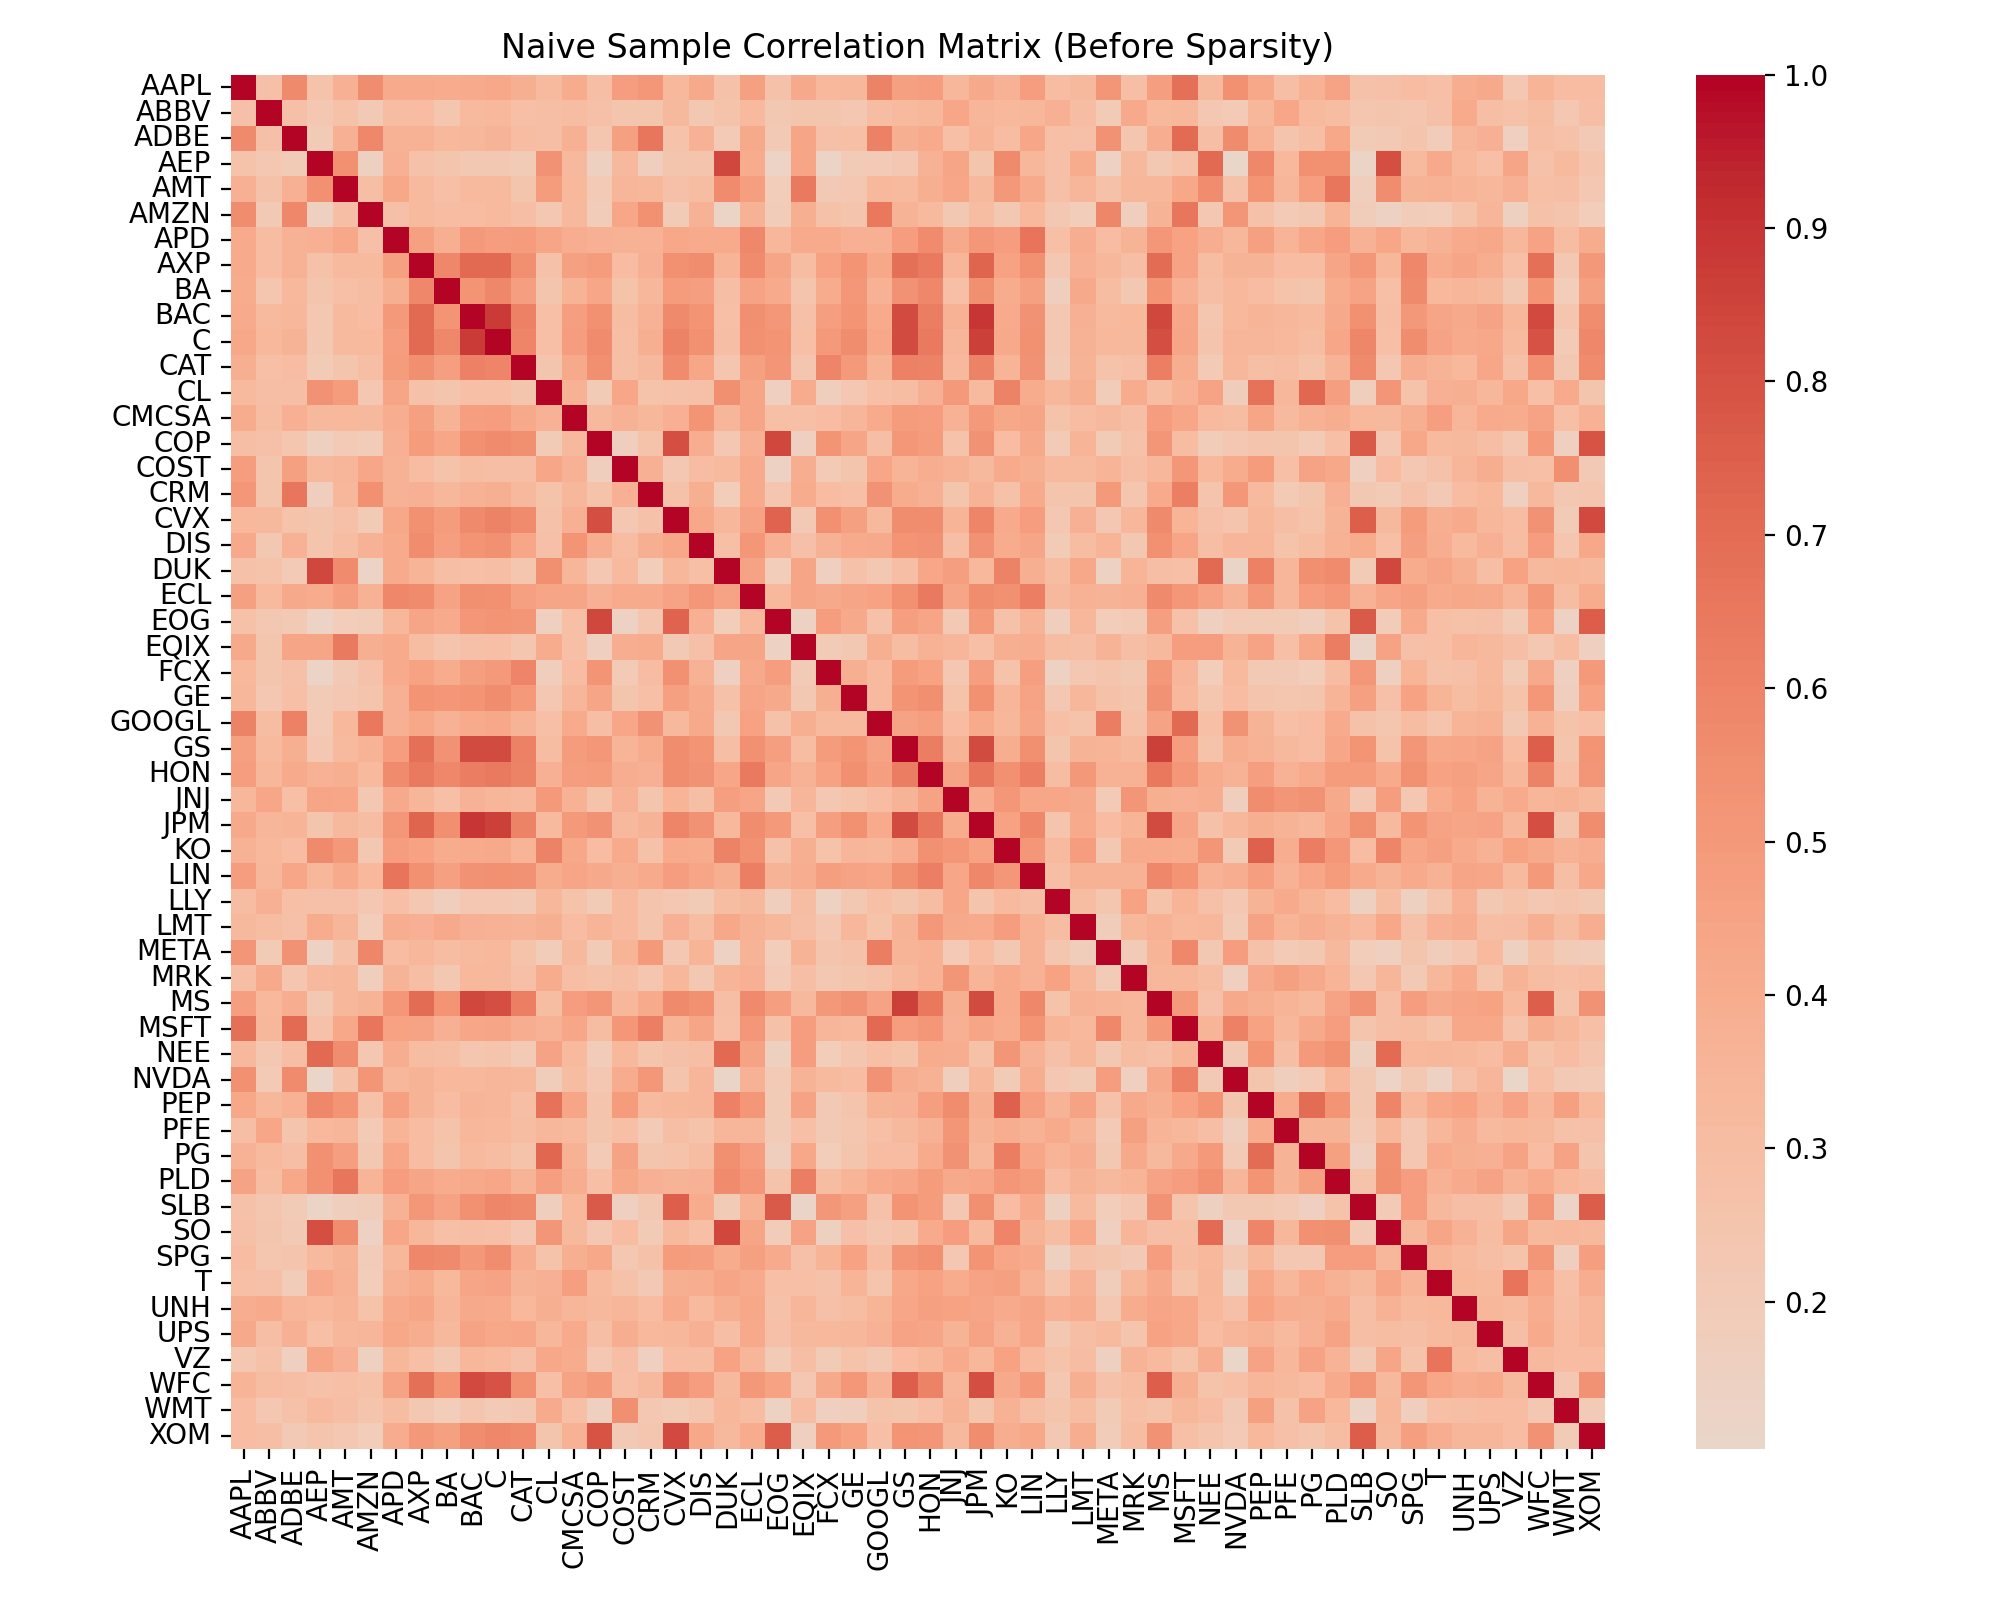
\includegraphics[width=0.8\textwidth]{../results/figures/01_correlation_heatmap.png}
    \caption{Naive sample correlation matrix across the asset universe.}
    \label{fig:heatmap}
\end{figure}

\subsection{Sparse Network Structure}
In stark contrast to the dense correlation matrix, the Graphical Lasso estimation yields a highly interpretable sparse network (Figure~\ref{fig:network}). The estimated network reveals clear sector-based clustering: Technology, Energy, and Financials form tightly interconnected conditional dependency clusters, while defensive sectors such as Healthcare and Consumer Staples remain largely conditionally independent, exhibiting minimal edges with the broader market. This topology aligns with financial theory, where defensive assets exhibit lower beta and weaker co-movement with cyclical sectors.

\begin{figure}[htbp]
    \centering
    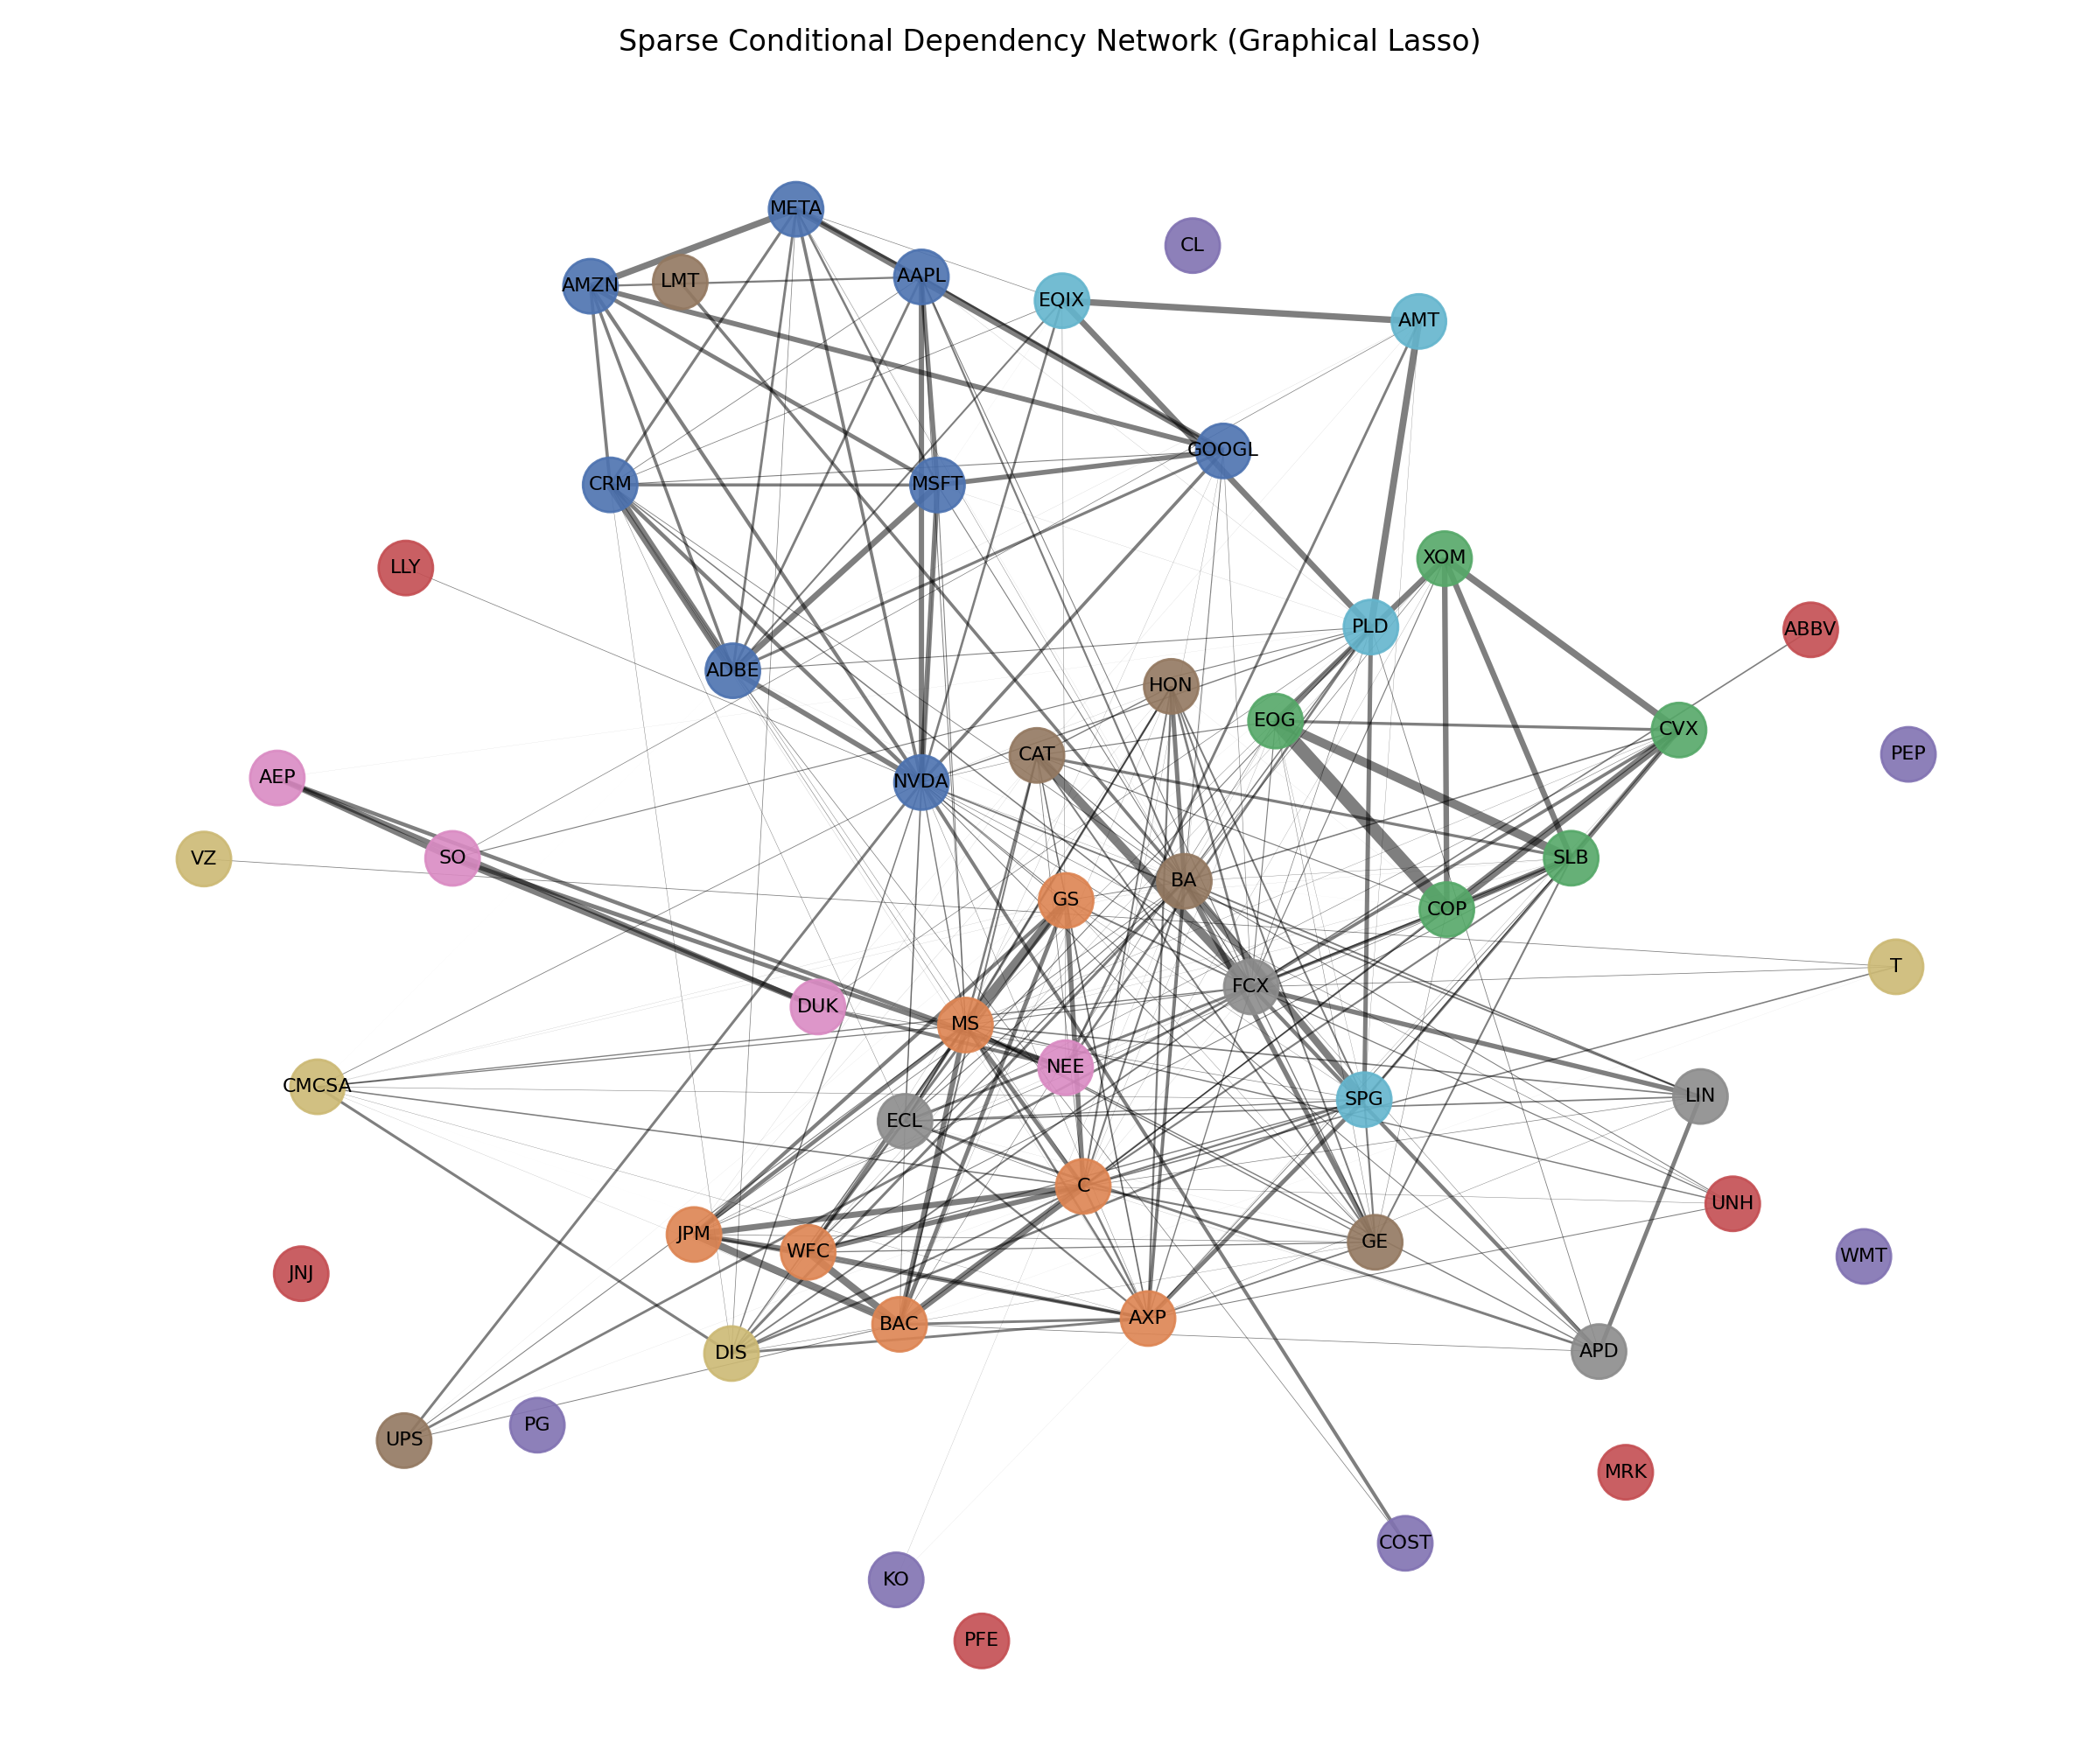
\includegraphics[width=0.85\textwidth]{../results/figures/02_sparse_network.png}
    \caption{Sparse conditional dependency network estimated via Graphical Lasso.}
    \label{fig:network}
\end{figure}

\subsection{Regime Comparison}
We split the $T = 2,514$ daily return observations into two equal temporal regimes ($T_A = 1,257$, $T_B = 1,257$) to evaluate structural invariance:
\begin{itemize}
    \item \textbf{Regime A (Pre-2020):} The estimated precision matrix yielded 195 non-zero off-diagonal edges.
    \item \textbf{Regime B (2020--Present):} The estimated precision matrix expanded to 266 edges (a 36.4\% increase in edge density).
\end{itemize}
The Jaccard similarity index between edge sets $E_A$ and $E_B$ is given by:
\begin{equation}
J(E_A, E_B) = \frac{|E_A \cap E_B|}{|E_A \cup E_B|} = 0.405
\end{equation}
This confirms a pronounced structural break and increased market coupling following the macroeconomic shocks of early 2020.

\subsection{Stability Selection}
To ensure edge persistence is not driven by finite-sample variance, we performed $B = 20$ bootstrap resamples. A total of \textbf{198 edges} satisfied a selection probability threshold of $\pi_{\text{thr}} \ge 0.80$, verifying that the core structure of the estimated networks represents robust, non-spurious dependencies.

\section{Discussion}
The estimated sparse network provides a refined view of market structure, isolating direct conditional dependencies from the dense web of indirect correlations inherent in the sample covariance matrix. The pronounced 36.4\% increase in edge density post-2020 suggests that during periods of systemic stress, market participants treat diverse assets as highly substitutable, leading to increased co-movement and reduced diversification benefits. The identification of 198 highly stable edges provides a robust foundation for downstream applications, such as constructing minimum-variance portfolios or monitoring financial contagion. 

However, this preliminary study has limitations. The static regime split at the year 2020 is inherently arbitrary and may not capture the exact timing of structural breaks. Furthermore, the assumption of temporal stationarity within each regime ignores the continuous, dynamic evolution of market dependencies. Finally, the regularization parameter $\lambda$ was selected via a fixed cross-validation scheme; future work could explore adaptive penalization or heterogeneous shrinkage to better accommodate varying edge strengths.

\section{Future Work}
Future research could extend this static framework to capture continuous market dynamics using Time-Varying Graphical Lasso (TVGL), which allows the precision matrix to evolve smoothly over time. Additionally, joint graphical lasso models could be employed to estimate networks across multiple regimes simultaneously, encouraging shared structure while allowing for regime-specific deviations. Finally, Bayesian sparse estimation techniques could provide posterior distributions for the edge weights, offering a natural measure of uncertainty for the estimated network topology.

\section{Conclusion}
This study applied sparse inverse covariance estimation to model the conditional dependency structure of 54 U.S. equities from 2015 to 2024. By employing the Graphical Lasso, we successfully extracted a sparse, interpretable network that avoids the instability and spurious correlations inherent in the sample covariance matrix.

Our regime comparison revealed a pronounced structural break: the post-2020 network exhibited a 36.4\% increase in edge density compared to the pre-2020 period, reflecting heightened systemic coupling during macroeconomic shocks. Furthermore, stability selection confirmed that the core topology of 198 edges is highly robust, representing non-spurious dependencies rather than finite-sample artifacts.

Ultimately, these robust, sparse conditional dependency networks offer a superior foundation for downstream financial applications, including systemic risk monitoring, financial contagion modeling, and mean-variance portfolio optimization.

\bibliographystyle{plainnat}
\bibliography{references}

\end{document}
